\documentclass[10pt]{report}

\usepackage{talks}
\newcommand{\expect}[1]{\mathbb{E}\!\left[ #1 \right]}
\newcommand{\reals}{\mathbb{R}}
\newcommand{\draw}[2]{#1^{(#2)}}
\usepackage{mathpazo}
\usepackage{sourcecodepro}
\usepackage{tikz}
    \usetikzlibrary{positioning, shapes, arrows.meta}

\newcommand{\ddfrac}[2]{\frac{\strut \displaystyle #1}{\strut \displaystyle #2}}
    
\begin{document}

\sf \mbox{}
\\[12pt]
\spc{\LARGE\bfseries \color{MidnightBlue}{50 years of word embeddings}}
\\[40pt]
\noindent 
\spc{\large\bfseries \color{MidnightBlue}{Bob Carpenter}}
\\[2pt]
\spc{\small Center for Computational Mathematics}
\\[-1pt]
\spc{\small Flatiron Institute}
\\[2pt]
\spc{\footnotesize \url{bcarpenter@flatironinstitute.org}}
\vfill 
\noindent 
\spc{\footnotesize December 2023 \qquad CCM Transformer Reading Group}
\hfill

\includegraphics[width=1.25in]{img/flatiron-logo.png}


\sld{What's a word embedding}
\begin{itemize}
\item Let $W$ be the \myemph{number of distinct words}.
\item Let $P$ be the \myemph{embedding dimension}.
\item Let   $[W] = \{ 0, \ldots, W - 1 \}$ be the set of words.
\item A \myemph{word embedding} is a function $f \, \textrm{:} \, [W] \rightarrow \mathbb{R}^P$.
\vfill
\item Assuming \myemph{finitely many words} is problematic
  \begin{subitemize}
  \item what's a word? (e.g., Chinese)
  \item productive morphology? (e.g., Turkish)
  \end{subitemize}
\end{itemize}

\sld{Document and query vectors for retrieval}
\begin{itemize}
\item Let $P = W$ (embedding dimension is number of words).
\item Use \myemph{one-hot embedding}, where $f(w) = v \in
  \mathbb{R}^W$ such that
  $$
  v_u = \begin{cases} 1 & \textrm{if } u = w \\ 0 & \textrm{otherwise} \end{cases}
  $$
\item Let $D$ be the number of documents.
\item Use \myemph{term frequency} document embedding $g$ defined by
  $g(d)_w$ is the count of word $w \in [W]$ in document $d \in [D]$,
  i.e., the sum of its word embeddings.
\end{itemize}
  
\sld{Document retrieval (cont.)}
\begin{itemize}
\item A \myemph{search query} $q$ is another sequence of words.
\item Score document $d$ for query $q$ using \myemph{cosine}
  between embedding vectors (lower angle is better),
  $$
  \textrm{dist}(d, q) = g(d)^{\top} \cdot g(q)
  $$
\end{itemize}
\vfill
\spc  {\small (Salton 1968)}

\sld{Inverse document frequency}
\begin{itemize}
\item The \myemph{document frequency} of a word is the number of
  documents in which it appears.
\item Intuition is rarer words more useful.
\item Embed documents by dividing word frequencies by their document
  frequency.
\item Resulting embedding is term-frequency/inverse document frequency
  (TF-IDF). 
\end{itemize}
\vfill
\spc {\small (Sp\"arck Jones 1972)}

\sld{Latent semantic analysis (LSA)}
\begin{itemize}
\item Take $W \times D$ TF-IDF matrix $X$ and singular value decompose,
  $$
  X = U \cdot \textrm{diagMat}(S) \cdot V^{\top},
  $$
  so $U$ and $V$ are orthonormal
\item Restrict to rank $K < \textrm{min}(D, W)$ by taking
  $X \approx U_{1:W,1:K} \cdot \textrm{diagMat}(S_{1:K}) \cdot V_{1:D,
    1:K}^{\top}$
\item Minimizes square error (``Mahalanobis'') at rank $K$
\item Use $U_{w,1:K}$ as document embedding and $V_{d,1:K}$ as
  document embedding (both embedded in $\mathbb{R}^K$).
\item Embed queries by \myemph{sum of word embeddings} and compare with cosine. 
\end{itemize}
\vfill
\spc {\small (Dumais, Furnas, Landauer, Deerwester 1988)}

\sld{Word embeddings for language modeling}
\begin{itemize}
\item Embed words.
\item Apply \myemph{hierarchical clustering} to the word embeddings.
\item Use classes from clusters to smooth $n$-gram language models.
\item This found all sorts of uses, including as covariate extractors
  for classification.
\end{itemize}
\vfill
\spc {\small (Peter Brown, Peter de Souza, Robert Mercer, Vincent Della
Pietra, Jenifer Lai, 1992)}


\sld{Pure text embeddings and skip-grams}
\begin{itemize}
\item Instead of word by documents, just use a corpus of text.
\item Model a word by frequencies of \myemph{words appearing around it}
  (i.e., the ``company it keeps'')
\item Allow skipping, dubbed a \myemph{skip-gram} (vs. contiguous
  \myemph{n-gram}).
\item Use like every other embedding.
  \vfill
  \spc {\small (Rosenfeld 1994), etc.}
  \\
  \spc {\small (Guthrie, Allison, Liu, Guthrie, Wilks 2006) \myemph{survey})}
\end{itemize}

\sld{Word embeddings as covariates}
\begin{itemize}
\item People used \myemph{word embeddings as predictors} in
  classifiers.
\item Map a query to the sum of the low-rank embeddings of its words.
\item For example, we used them in \myemph{logistic regression} for call routing
  (target modeled as sum of training queries)
\\ \qquad {\footnotesize Chu-Caroll, Carpenter. 1999. Vector-based natural 
    language call routing. \textit{CL}.}
\item We also used them to \myemph{disambiguate ambiguous queries}
  (e.g., difference of destination embedding vectors minus query)
  \\
  \qquad {\footnotesize Bob Carpenter and Jennifer Chu-Carroll. 2001. Methods and
  apparatus for automatic call routing including disambiguating
  routing decisions. \textit{U.S.\ Patent} \# 6269153.}
\end{itemize}

\sld{Word2Vec}
\begin{center}
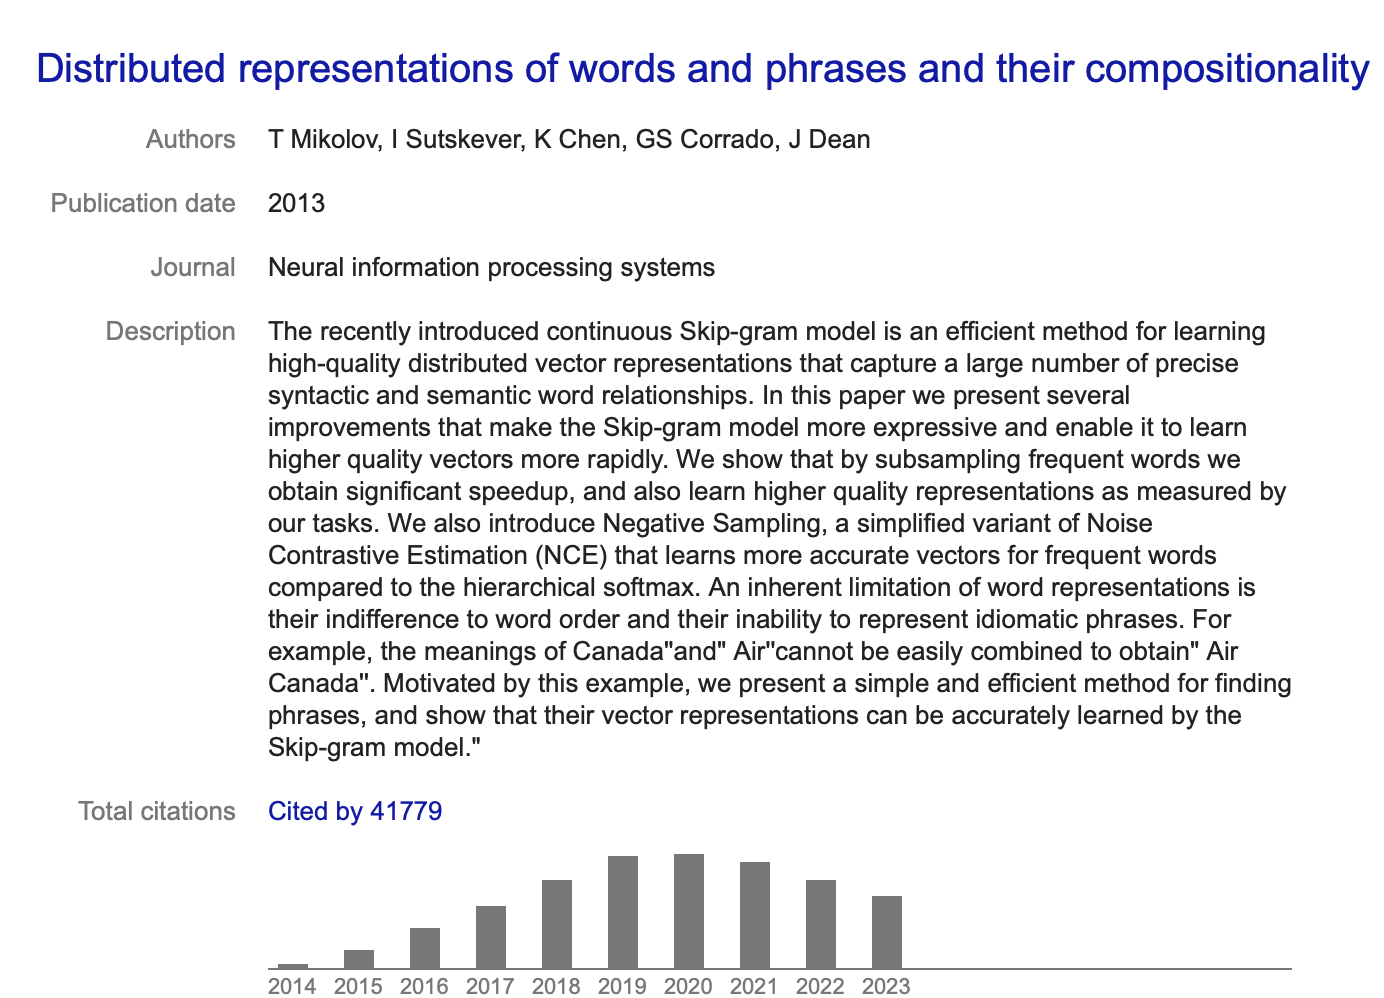
\includegraphics[width=2.5in]{img/word2vec.png}
\end{center}
\vfill
\spc {\small (Mikolov, Sutskever, Chen, Corrado, Dean 2013)}

\sld{What is Word2Vec?}
\begin{itemize}
\item Skip-grams trained with a \myemph{neural network}.
\item \myemph{Large-scale} training.
\item \myemph{Open-source} software.
  \vfill
\item \myemph{Superseded} by transformer embeddings
  \begin{subitemize}
  \item embeddings \myemph{jointly optimized} with other parameters
  \end{subitemize}
\end{itemize}

\end{document}
